\documentclass[aspectratio=169]{../latex_main/tntbeamer}  % you can pass all options of the beamer class, e.g., 'handout' or 'aspectratio=43'
\usepackage{dsfont}
\usepackage{bm}
\usepackage[english]{babel}
\usepackage[T1]{fontenc}
%\usepackage[utf8]{inputenc}
\usepackage{graphicx}
\graphicspath{ {./figures/} }
\usepackage{algorithm}
\usepackage[ruled,vlined,algo2e,linesnumbered]{algorithm2e}
\usepackage{hyperref}
\usepackage{booktabs}
\usepackage{mathtools}

\usepackage{amsmath,amssymb}

\DeclareMathOperator*{\argmax}{arg\,max}
\DeclareMathOperator*{\argmin}{arg\,min}

\usepackage{pgfplots}
\pgfplotsset{compat=1.16}
\usepackage{tikz}
\usetikzlibrary{trees} 
\usetikzlibrary{shapes.geometric}
\usetikzlibrary{positioning,shapes,shadows,arrows,calc,mindmap}
\usetikzlibrary{positioning,fadings,through}
\usetikzlibrary{decorations.pathreplacing}
\usetikzlibrary{intersections}
\pgfdeclarelayer{background}
\pgfdeclarelayer{foreground}
\pgfsetlayers{background,main,foreground}
\tikzstyle{activity}=[rectangle, draw=black, rounded corners, text centered, text width=8em]
\tikzstyle{data}=[rectangle, draw=black, text centered, text width=8em]
\tikzstyle{myarrow}=[->, thick, draw=black]

% Define the layers to draw the diagram
\pgfdeclarelayer{background}
\pgfdeclarelayer{foreground}
\pgfsetlayers{background,main,foreground}

% Requires XeLaTeX or LuaLaTeX
\usepackage{unicode-math}

\usepackage{fontspec}
%\setsansfont{Arial}
\setsansfont{RotisSansSerifStd}[ 
Path=../latex_main/fonts/,
Extension = .otf,
UprightFont = *-Regular,  % or *-Light
BoldFont = *-ExtraBold,  % or *-Bold
ItalicFont = *-Italic
]
\setmonofont{Cascadia Mono}[
Scale=0.8
]

% scale factor adapted; mathrm font added (Benjamin Spitschan @TNT, 2021-06-01)
%\setmathfont[Scale=1.05]{Libertinus Math}
%\setmathrm[Scale=1.05]{Libertinus Math}

% other available math fonts are (not exhaustive)
% Latin Modern Math
% XITS Math
% Libertinus Math
% Asana Math
% Fira Math
% TeX Gyre Pagella Math
% TeX Gyre Bonum Math
% TeX Gyre Schola Math
% TeX Gyre Termes Math

% Literature References
\newcommand{\lit}[2]{\href{#2}{\footnotesize\color{black!60}[#1]}}

%%% Beamer Customization
%----------------------------------------------------------------------
% (Don't) Show sections in frame header. Options: 'sections', 'sections light', empty
\setbeamertemplate{headline}{empty}

% Add header logo for normal frames
\setheaderimage{
	% 
\includegraphics[height=\logoheight]{figures/TNT_darkv4.pdf}
	
\includegraphics[height=\logoheight]{../latex_main/figures/luh_logo_rgb_0_80_155.pdf}
	% 
\includegraphics[height=\logoheight]{figures/logo_tntluh.pdf}
}

% Header logo for title page
\settitleheaderimage{
	% 
\includegraphics[height=\logoheight]{figures/TNT_darkv4.pdf}
	
\includegraphics[height=\logoheight]{../latex_main/figures/luh_logo_rgb_0_80_155.pdf}
	% 
\includegraphics[height=\logoheight]{figures/logo_tntluh.pdf}
}

% Title page: tntdefault 
\setbeamertemplate{title page}[tntdefault]  % or luhstyle
% Add optional title image here
%\addtitlepageimagedefault{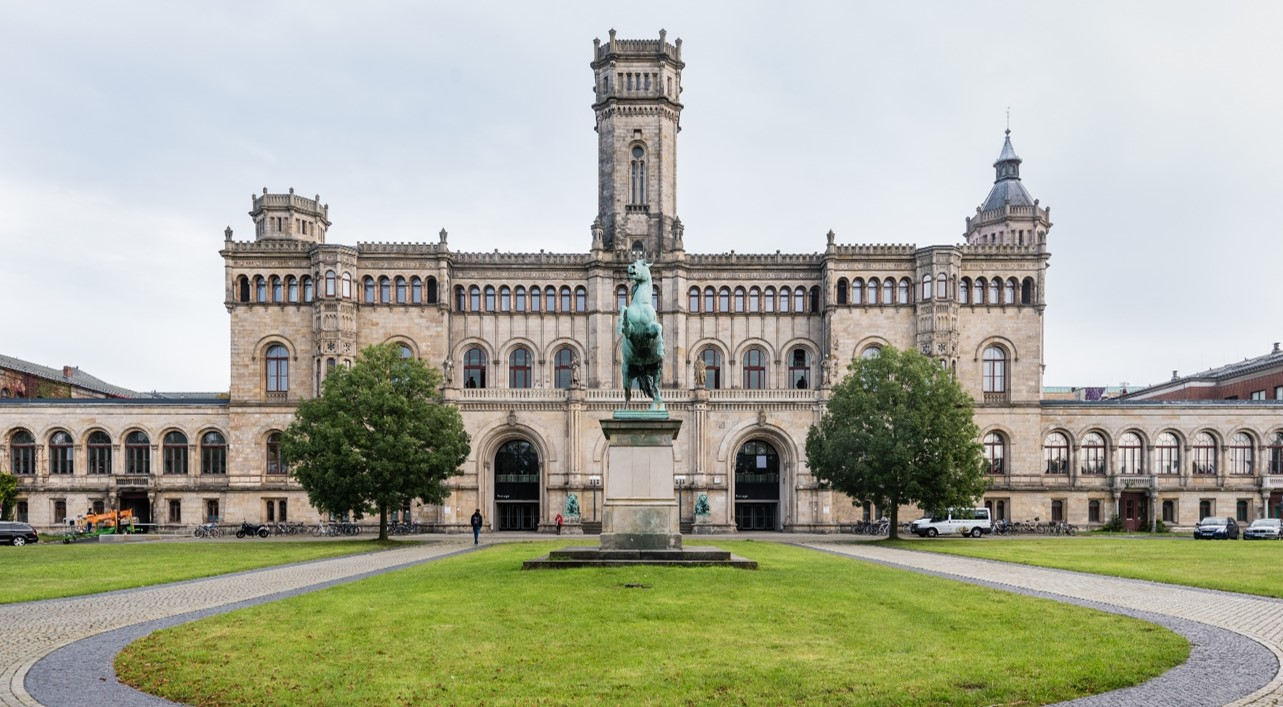
\includegraphics[width=0.65\textwidth]{figures/luh_default_presentation_title_image.jpg}}

% Title page: luhstyle
% \setbeamertemplate{title page}[luhstyle]
% % Add optional title image here
% \addtitlepageimage{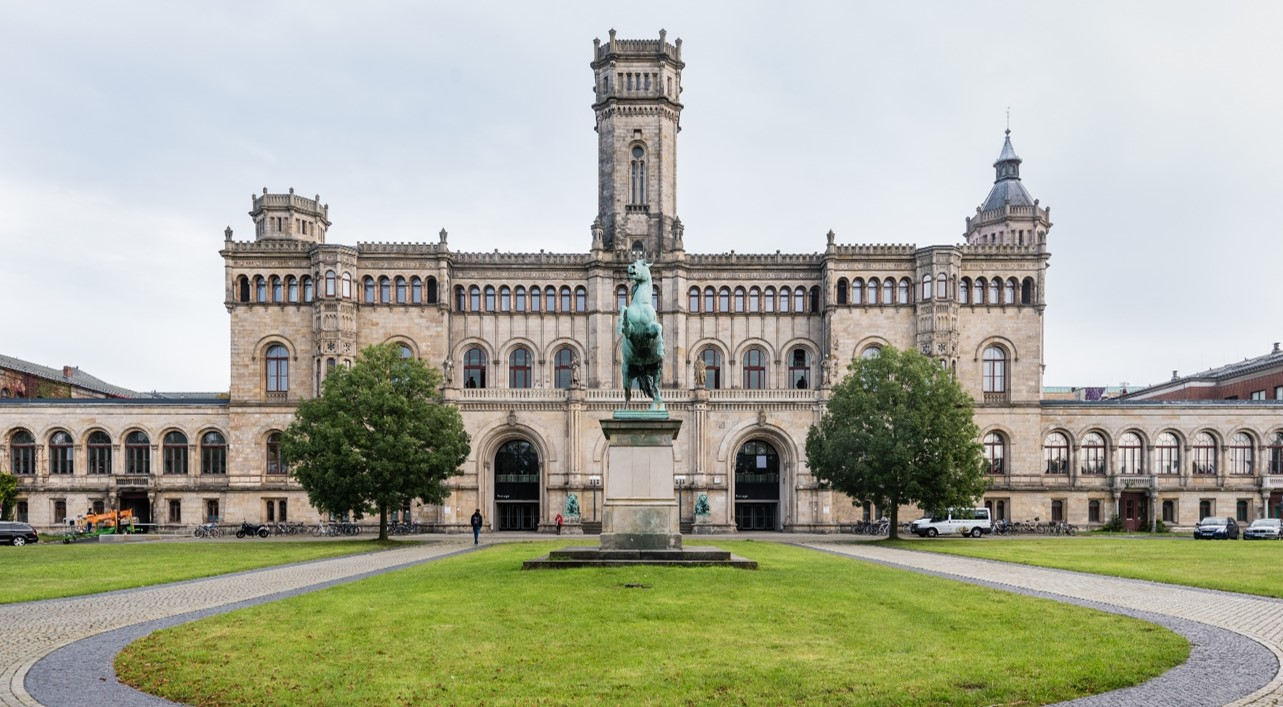
\includegraphics[width=0.75\textwidth]{figures/luh_default_presentation_title_image.jpg}}

\author[Lindauer \& Anand]{Marius Lindauer and Avishek Anand\\[1em]
	
\includegraphics[height=\logoheight]{../latex_main/figures/luh_logo_rgb_0_80_155.pdf}\qquad

\includegraphics[height=\logoheight]{../latex_main/figures/TNT_darkv4}\qquad

\includegraphics[height=\logoheight]{../latex_main/figures/L3S.jpg}	}
\date{Winter Term 2021
}


%%% Custom Packages
%----------------------------------------------------------------------
% Create dummy content
\usepackage{blindtext}

% Adds a frame with the current page layout. Just call \layout inside of a frame.
\usepackage{layout}


\title[Introduction]{iML: Local Explanations}
\subtitle{LIME}

%\institute{}


\begin{document}
	
	\maketitle

	%-----------------------------------------------------------------------------------------------------------------------------


\begin{frame}{LIME}
\begin{itemize}
		\item Local Interpretable Model-agnostic Explanations (LIME) assume that even if a machine learning model is very complex, \alert{the local prediction can be described with a simpler model}.
		\smallskip\pause
		\item  Therefore, LIME explains \textbf{individual} predictions of \textbf{any} black-box model by approximating the model \textbf{locally} with an interpretable model.
		\smallskip\pause
		\item These approximations are called local surrogate models.\\ Typically, they are linear models or trees.
		\smallskip\pause
		\item They should answer why a machine learning model predicted $y$ for input $x$.
		\smallskip\pause
		\item Since they can be applied to any black-box model they are model-agnostic.  
		\smallskip\pause
		\item They can handle tabular, image and text data. 
\end{itemize}
\end{frame}
%----------------------------------------------
\begin{frame}[c]{Formal Definition}
	LIME provides a local explanation for a black-box model $\hat{f}$ in form of a model $g \in \mathcal{G}$ with $\mathcal{G}$ as the class of potential (interpretable) models. This model $g$ should have two characteristics:
	\begin{enumerate}
		\item It should be \textbf{interpretable}, i.e. provide qualitative understanding between the input variables and the response that are easy to understand.  
		\item It should be \textbf{locally faithful}, i.e. it should behave similarly to $\hat{f}$ in the vicinity of the instance being predicted. This characteristic is also called local fidelity. 
	\end{enumerate}
	Formally, we want to receive a model $g$ with minimal complexity and maximal local-fidelity. 
\end{frame}
%----------------------------------------------
\begin{frame}{Model Complexity}
We can measure the complexity of a model $g$ using $J(g)$. \\ 
\vspace{0.5cm}
 	\textbf{Example: Linear model}\\
 	Let $\mathcal{G} = \left\{g: \mathcal{X} \to \mathbb{R} ~|~g(x) = s(w^\top x)\right\}$ be the class of linear models with $s(\cdot)$ being either the identity function for linear regression or the logistic sigmoid function for logistic regression. \\
 	Then, $J(g) = \sum_{j = 1}^p \mathrm{I}_{\{ w_j \neq 0 \}}$ could be the L$_0$ loss, i.e. the number of non-zero coefficients. 
 	\vspace{0.5cm}
 	
 	\textbf{Example: Tree}\\
 	Let $\mathcal{G} = \left\{g:\mathcal{X} \to \mathbb{R} ~|~g(x) = \sum_{m=1}^M c_m \mathrm{I}_{\{ x \in Q_m \}}\right\}$ be the class of trees (i.e., class of additive model over the leaf-rectangles) then $J(g)$ could measure the number of terminal/leaf nodes.\\
 \end{frame}

 %----------------------------------------------
\begin{frame}{Local Model Fidelity}
\vspace{-2em}
 		\begin{itemize}
 			\item A model $g$ is locally faithful to $\hat{f}$ w.r.t. a point $x$\\ if for points $z \in \mathcal{Z} \subseteq \mathbb{R}^p$ close to $x$, the predictions of $g(z)$ are close to $\hat{f}(z)$. 
 			\pause
 			 \item In an optimization task: the closer $z$ is to $x$, the closer $g(z)$ should be to $\hat{f}(z)$.  
 			 \pause
 			\item For this definition we need two measures:
 			\begin{enumerate}
 				\item A proximity measure $n(z)$ between $z$ and $x$, e.g. the exponential kernel
 				$$n(z) = exp(-d(x, z)^2/\sigma^2)$$ 
 				with $\sigma$ as the kernel width. $d$ could be for example the Euclidean distance for numeric features. 
 				\pause
 				\item A distance measure or loss function $L(\hat{f}(z), g(z))$ to assess how close the predictions of $\hat{f}(z)$ and $g(z)$ are, e.g. the L2 loss/squared error $$L(\hat{f}(z), g(z)) = (g(z) - \hat{f}(z))^2.$$ 
 			\end{enumerate}
 			\pause
 			\item Given points $z$, we can measure local fidelity of $g$ with respect to $\hat{f}$ in terms of a weighted loss
 			\begin{equation}
 				L(\hat{f}, g, n) = \sum_{z \in \mathcal{Z}} n(z) L(\hat{f}(z), g(z))
 				\label{eq:optim}
 			\end{equation}
 			%\item Note that identifying \textbf{locally} faithful explanations that are interpretable is less of a challenge than identifying \textbf{globally} faithful explanations. Yet, global fidelity implies local fidelity but not vice versa.
 		\end{itemize}
\end{frame}
%----------------------------------------------
\begin{frame}{Minimization task}
	\begin{itemize}
		\item Formally, an explanation produced by LIME is obtained by the following: 
		$$ \argmin_{g \in \mathcal{G}} L(\hat{f}, g, n) + J(g)$$
		\item In practice, LIME only optimizes $L(\hat{f}, g, n)$ (model-fidelity). 	
		\item The model complexity ($J(g)$) is determined by users beforehand by restricting the class $\mathcal{G}$. For example, users could only consider sparse linear models. 
		\item Since we want a \textbf{model-agnostic} explainer, we need to optimize $L(\hat{f}, g, n)$ without making any assumptions about $\hat{f}$. 
		\item Therefore, we learn $g$ only approximately with the following algorithm.  
		\end{itemize}
\end{frame} 
%----------------------------------------------
\begin{frame}{LIME Algorithm \lit{Ribeiro et al. 2016}{https://arxiv.org/abs/1602.04938}}
    \vspace{-1em}
		For the algorithm, we need a pre-trained model $\hat{f}$, $x$ whose prediction we want to explain and model class $\mathcal{G}$.\\ \vspace{0.5cm}
		We illustrate the steps of the algorithm with a classification example: 
		\begin{itemize}
			\item The light/dark background represents the prediction surface of a \alert{classifier} $\hat{f}: \mathbb{R}^2 \to \{0, 1\}$.
			\item The yellow point displays $x$ we are interested in. 
			\item $\mathcal{G}$ is restricted to the class of logistic regression models ($\to$ classification). 
		\end{itemize}
		\begin{center}
			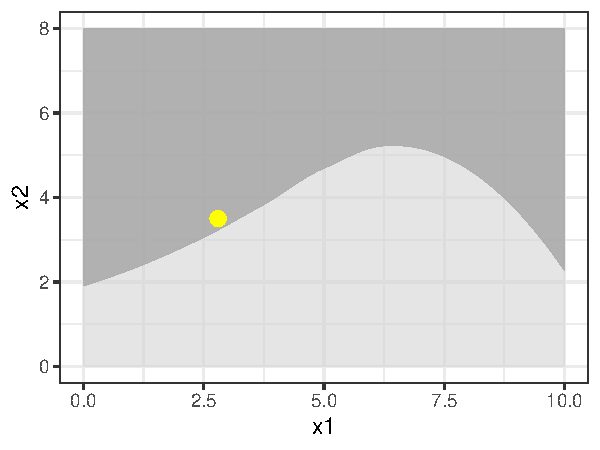
\includegraphics[width=0.3\textwidth]{figure/lime2}
		\end{center}

\end{frame}
%----------------------------------------------
\begin{frame}{LIME Algorithm \lit{Ribeiro et al. 2016}{https://arxiv.org/abs/1602.04938}}

        \vspace{-2em}	
		\begin{enumerate}
		\item Independently sample new points $z \in \mathcal{Z}$. 
		\item Retrieve predictions $\hat{f}(z)$ for obtained points $z$. \\[0.2cm]
		
		\hspace{-0.7cm} Strategies for sampling: 
		\begin{itemize} 
			\item Uniformly sample new points from the feasible feature range. 
			\item Use the training data set with or without perturbations.
			\item Draw samples from the estimated univariate distribution of each feature.
			\item Create an equidistant grid over the supported feature range.  
		\end{itemize}
		\begin{center}
			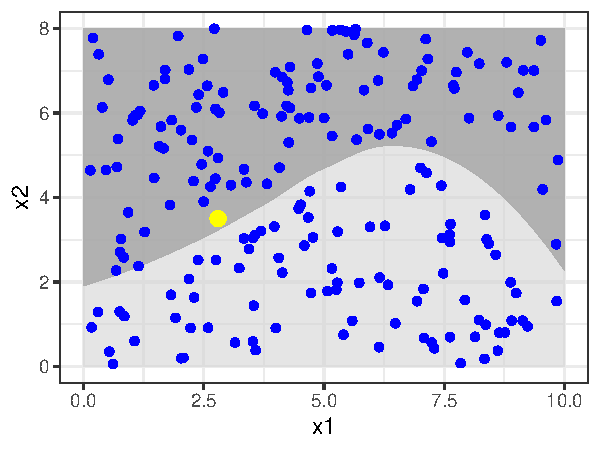
\includegraphics[width=0.3\textwidth]{figure/lime3} \hspace{0.1cm}
			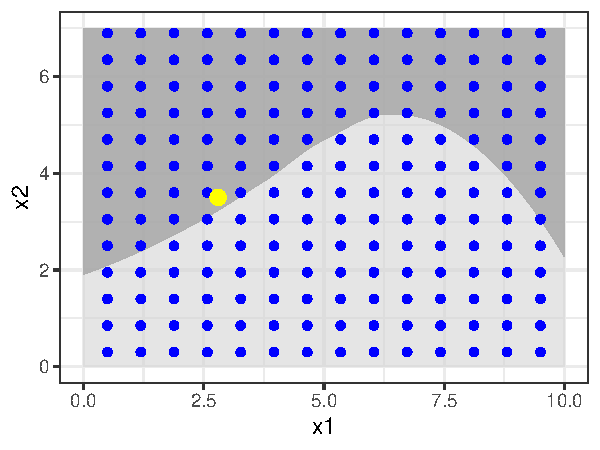
\includegraphics[width=0.3\textwidth]{figure/lime3a}
		\end{center}
		\item Weight $z \in \mathcal{Z}$ by their proximity $n(z)$.
		\\[0.2cm]
		\end{enumerate}

\end{frame}
%----------------------------------------------
\begin{frame}{LIME Algorithm \lit{Ribeiro et al. 2016}{https://arxiv.org/abs/1602.04938}}

		In this example, we use the exponential kernel defined on the Euclidean distance $d$
		 $$n(z) = exp(-d(x, z)^2/\sigma^2).$$ 
		\begin{center}
			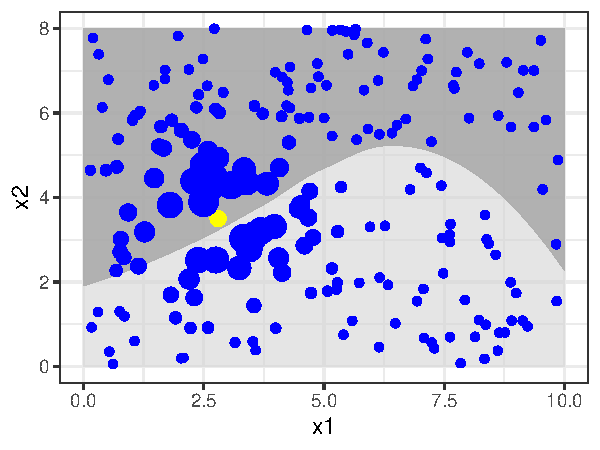
\includegraphics[width=0.4\textwidth]{figure/lime4}
		\end{center}
% 	An alternative is the Gower proximity: 
% 	$n(z) = 1 - \Gower(z, x) =  1 - \frac{1}{p}\sum_{j = 1}^{p} \delta_G(z_j, x_j) $ 
% 	$\textnormal{ with } \delta_G(z_j, x_j) = 
% 	\begin{cases}
% 	\frac{1}{\widehat{R}_j}|z_j- x_j| & \text{if $x_j$ and $z_j$ are numerical} \\
% 	\mathbb{I}_{z_j \neq x_j} & \text{if $x_j$ and $z_j$) are categorical.}
% 	\end{cases}$
		

\end{frame}
%----------------------------------------------
\begin{frame}{LIME Algorithm \lit{Ribeiro et al. 2016}{https://arxiv.org/abs/1602.04938}}
		\begin{enumerate}
			\setcounter{enumi}{3}
		\item Train a interpretable model $g$ on weighted data points $z \in \mathcal{Z}$. The obtained predictions $\hat{f}(z)$ is the target of this model.
		\item Return the interpretable model $g$ as the explainer. \\[0.3cm]
			\end{enumerate}
		Popular interpretable models are linear models, LASSO, classification/regression trees, decision rules. \\
		In our example, we fit a logistic regression model. \\Consequently, $L(\hat{f}(z), g(z))$  is the Bernoulli loss in Eq.~(\ref{eq:optim}). 
		\begin{center}
			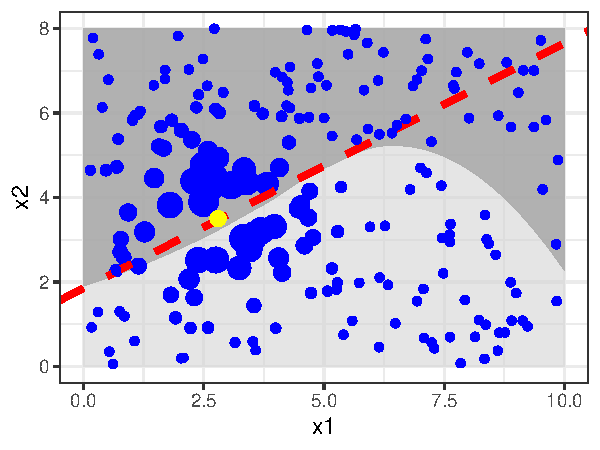
\includegraphics[width=0.3\textwidth]{figure/lime5}
		\end{center}
\end{frame}



\end{document}